\documentclass[11pt,a4paper]{ctexart}

\usepackage{amsmath,amssymb,bm}
\usepackage{geometry}
\usepackage{enumitem}
\usepackage{fancyhdr}
\usepackage{lastpage}
\usepackage{xcolor}
\usepackage{tcolorbox}
\usepackage{tikz}
\usepackage{titlesec}
\usepackage{microtype}
\usetikzlibrary{arrows.meta,calc}

\geometry{left=2.15cm,right=2.15cm,top=2.0cm,bottom=2.0cm}
\setlength{\parindent}{2em}
\setlength{\parskip}{0.25em}
\linespread{1.12}

\definecolor{mainblue}{RGB}{39,91,150}
\definecolor{lightblue}{RGB}{232,241,252}
\definecolor{darkgray}{RGB}{65,65,65}
\definecolor{lightgray}{RGB}{245,246,248}

\titleformat{\section}{\large\bfseries\color{mainblue}}{}{0em}{}[\titlerule]
\titleformat{\subsection}{\normalsize\bfseries\color{darkgray}}{}{0em}{}
\titlespacing*{\section}{0pt}{0.9em}{0.45em}
\titlespacing*{\subsection}{0pt}{0.65em}{0.25em}

\setlist[enumerate]{leftmargin=2.2em,itemsep=0.25em,topsep=0.25em}
\setlist[itemize]{leftmargin=2.0em,itemsep=0.2em,topsep=0.2em}

\pagestyle{fancy}
\fancyhf{}
\lhead{\small 格物助航｜每日一练}
\rhead{\small 2026.6.6}
\cfoot{\small 第 \thepage\ 页 / 共 \pageref{LastPage} 页}
\renewcommand{\headrulewidth}{0.4pt}

\newtcolorbox{problemBox}{
  colback=lightblue,
  colframe=mainblue,
  arc=2mm,
  boxrule=0.7pt,
  left=1.0em,
  right=1.0em,
  top=0.8em,
  bottom=0.8em,
  before skip=0.6em,
  after skip=0.8em
}

\newtcolorbox{tipBox}{
  colback=lightgray,
  colframe=darkgray,
  arc=1.5mm,
  boxrule=0.5pt,
  left=0.9em,
  right=0.9em,
  top=0.6em,
  bottom=0.6em,
  before skip=0.5em,
  after skip=0.5em
}

\newcommand{\dd}{\mathrm{d}}
\newcommand{\ii}{\bm{i}}
\newcommand{\jj}{\bm{j}}

\begin{document}

\begin{center}
  {\Large\bfseries\color{mainblue} 格物助航｜每日一练}\par
  \vspace{0.25em}
  {\large 力学第一章：质点运动学}\par
  \vspace{0.35em}
  {\small 2026年6月6日}
  \vspace{0.35em}
  {\small 编写：贡泽轩}
\end{center}

\vspace{-0.3em}

\begin{problemBox}
\noindent\textbf{题目}\quad
半径为 $R$ 的车轮在水平地面上向右作无滑动纯滚动，轮心以恒定速度向右运动，车轮角速度大小为 $\omega$。取地面为参考系，建立直角坐标系 $Oxy$，$x$ 轴沿地面向右，$y$ 轴竖直向上。设 $t=0$ 时，轮缘上一点 $P$ 正好与地面接触，并取该接触点为坐标原点。令 $\theta=\omega t$。求：
\begin{enumerate}
  \item 点 $P$ 在地面参考系中的运动方程；
  \item 点 $P$ 的速度 $\bm v$、加速度 $\bm a$ 以及速率 $v$；
  \item 在 $0<\theta<2\pi$ 内，点 $P$ 的切向加速度大小 $a_\tau$、法向加速度大小 $a_n$ 和轨迹曲率半径 $\rho$；
  \item 当 $P$ 运动到最高点时，求 $v$、$\bm a$、$a_\tau$、$a_n$ 和 $\rho$。
\end{enumerate}
\end{problemBox}

\begin{center}
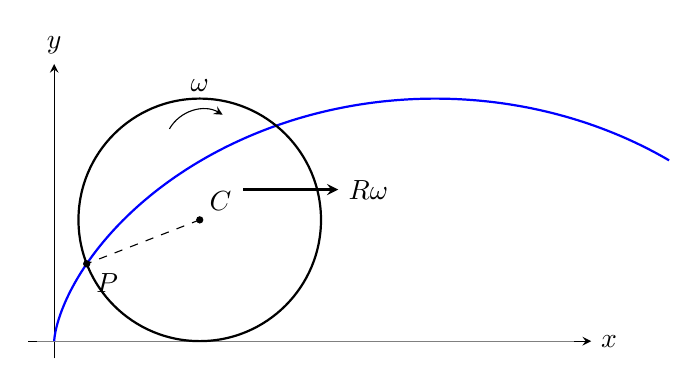
\begin{tikzpicture}[scale=1.1,>=stealth]
    % 参数
    \def\R{1.4}
    \def\th{1.2} % 当前转角 theta

    % 关键点
    \coordinate (O) at (0,0);
    \coordinate (C) at ({\R*\th},{\R});
    \coordinate (P) at ({\R*(\th-sin(\th r))},{\R*(1-cos(\th r))});

    % 坐标轴
    \draw[->] (-0.3,0) -- (6.2,0) node[right] {$x$};
    \draw[->] (0,-0.2) -- (0,3.2) node[above] {$y$};

    % 地面
    \draw[gray] (-0.2,0) -- (6.0,0);

    % 摆线轨迹
    \draw[blue, thick, domain=0:4.2, samples=200, smooth]
        plot ({\R*(\x - sin(\x r))},{\R*(1 - cos(\x r))});

    % 车轮
    \draw[thick] (C) circle (\R);

    % 轮心
    \fill (C) circle (1.2pt);
    \node[above right] at (C) {$C$};

    % 半径 CP
    \draw[dashed] (C) -- (P);

    % 点 P
    \fill (P) circle (1.2pt);
    \node[below right] at (P) {$P$};

    % 轮心速度箭头
    \draw[->, thick] ({\R*\th+0.5},{\R+0.35}) -- ({\R*\th+1.6},{\R+0.35})
        node[right] {$R\omega$};

    % 转动方向箭头（顺时针）
    \draw[->] ({\R*\th-0.35},{\R+1.05}) arc[start angle=150,end angle=60,radius=0.45];
    \node at ({\R*\th},{\R+1.55}) {$\omega$};

\end{tikzpicture}
\end{center}

\section*{详细解法}

\subsection*{一、求运动方程}

纯滚动可以看成轮心的平动，和点 $P$ 相对轮心的圆周运动的叠加。由无滑动的条件可得
\[
  x_C=R\theta=R\omega t,\qquad y_C=R.
\]
因此
\[
  \bm r_C=R\omega t\,\ii+R\,\jj .
\]
在轮心参考系中，$t=0$ 时 $P$ 在轮心正下方，所以
\[
  \bm r_{P/C}=-R\sin\theta\,\ii-R\cos\theta\,\jj .
\]
由相对运动的位置关系
\[
  \bm r_P=\bm r_C+\bm r_{P/C},
\]
得
\[
  \bm r_P=R(\theta-\sin\theta)\ii+R(1-\cos\theta)\jj .
\]
故点 $P$ 的运动方程为
\[
  \boxed{
  \begin{cases}
  x=R(\omega t-\sin\omega t),\\[0.2em]
  y=R(1-\cos\omega t).
  \end{cases}}
\]
这是一条\textbf{摆线}。

\subsection*{二、求速度、加速度与速率}

对运动方程求导：
\[
  v_x=\frac{\dd x}{\dd t}=R\omega(1-\cos\theta),
  \qquad
  v_y=\frac{\dd y}{\dd t}=R\omega\sin\theta.
\]
所以
\[
  \boxed{\bm v=R\omega(1-\cos\theta)\ii+R\omega\sin\theta\,\jj.}
\]
继续求导：
\[
  a_x=R\omega^2\sin\theta,
  \qquad
  a_y=R\omega^2\cos\theta.
\]
因此
\[
  \boxed{\bm a=R\omega^2\sin\theta\,\ii+R\omega^2\cos\theta\,\jj,}
  \qquad
  \boxed{a=R\omega^2.}
\]
由速率是速度矢量的大小，可得：
\[
\begin{aligned}
  v&=\sqrt{v_x^2+v_y^2}  \\
   &=R\omega\sqrt{(1-\cos\theta)^2+\sin^2\theta} \\
   &=R\omega\sqrt{2-2\cos\theta}
    =2R\omega\left|\sin\frac{\theta}{2}\right|.
\end{aligned}
\]
在 $0<\theta<2\pi$ 内，$\sin(\theta/2)>0$，于是
\[
  \boxed{v=2R\omega\sin\frac{\theta}{2}.}
\]

\subsection*{三、求切向加速度、法向加速度与曲率半径}

切向加速度描述速率大小的变化：
\[
  a_\tau=\frac{\dd v}{\dd t}.
\]
由 $v=2R\omega\sin(\theta/2)$ 与 $\theta=\omega t$，得
\[
  \boxed{a_\tau=R\omega^2\cos\frac{\theta}{2}.}
\]
自然坐标系中有
\[
  a^2=a_\tau^2+a_n^2.
\]
于是
\[
\begin{aligned}
  a_n&=\sqrt{a^2-a_\tau^2}  \\
     &=R\omega^2\sqrt{1-\cos^2\frac{\theta}{2}}
      =\boxed{R\omega^2\sin\frac{\theta}{2}}.
\end{aligned}
\]
又因为
\[
  a_n=\frac{v^2}{\rho},
\]
所以
\[
  \rho=\frac{v^2}{a_n}
  =\frac{4R^2\omega^2\sin^2(\theta/2)}{R\omega^2\sin(\theta/2)}
  =\boxed{4R\sin\frac{\theta}{2}}.
\]

\subsection*{四、求最高点处的物理量}

最高点对应 $\theta=\pi$。代入以上结果：
\[
  \boxed{v=2R\omega,}
  \qquad
  \boxed{\bm a=-R\omega^2\jj.}
\]
此时加速度竖直向下，指向轮心。并且
\[
  \boxed{a_\tau=0,\qquad a_n=R\omega^2,
  \qquad \rho=4R.}
\]

\section*{技巧与知识点}

\begin{tipBox}
\begin{enumerate}
  \item \textbf{相对运动思想：}把轮缘点的运动拆成轮心平动和相对轮心转动，先写出
  \[
    \bm r_P=\bm r_C+\bm r_{P/C}.
  \]
  速度和加速度可进一步求导而得。
  \item \textbf{由运动方程求运动学量：}已知 $\bm r(t)$，就用
  \[
    \bm v=\frac{\dd\bm r}{\dd t},\qquad
    \bm a=\frac{\dd\bm v}{\dd t}.
  \]
  \item \textbf{速度不等于速率：}$\bm v$ 是矢量，$v=|\bm v|$ 是标量。
  \item \textbf{曲线运动的加速度分解：}
  \[
    a_\tau=\frac{\dd v}{\dd t},
    \qquad
    a_n=\frac{v^2}{\rho}.
  \]
  \item \textbf{高频易错点：}一般曲线运动中，总加速度大小 $a$ 通常不等于 $\dd v/\dd t$；后者只是切向加速度。
\end{enumerate}
\end{tipBox}

\section*{复习建议}

第一章的知识点复习流程建议：
\[
  \text{运动方程}
  \longrightarrow
  \text{速度}
  \longrightarrow
  \text{加速度}
  \longrightarrow
  \text{速率}
  \longrightarrow
  \text{切向/法向分解}.
\]
建议重点练三类题：
\begin{enumerate}
  \item 已知 $x(t),y(t)$ 或 $\bm r(t)$，求轨迹、速度、加速度；
  \item 圆周运动和一般曲线运动，尤其是 $a_\tau$ 与 $a_n$ 的区分；
  \item 相对运动和纯滚动问题，尤其要熟悉“牵连量+相对量”的分解方法。
\end{enumerate}

\end{document}
